\documentclass[a4paper,11pt]{article}
\usepackage{amsmath,amsthm,amsfonts,amssymb,amscd,amstext,vmargin,graphics,graphicx,tabularx,multicol} 
\usepackage[francais]{babel}
\usepackage[utf8]{inputenc}  
\usepackage[T1]{fontenc} 
\usepackage{pstricks-add,tikz,tkz-tab,variations}
\usepackage[autolanguage,np]{numprint} 

\setmarginsrb{1.5cm}{0.5cm}{1cm}{0.5cm}{0cm}{0cm}{0cm}{0cm} %Gauche, haut, droite, haut
\newcounter{numexo}
\newcommand{\exo}[1]{\stepcounter{numexo}\noindent{\bf Exercice~\thenumexo} : \marginpar{\hfill /#1}}
\reversemarginpar

\newcommand{\bmul}[1]{\begin{multicols}{#1}}
\newcommand{\emul}{\end{multicols}}

\newcounter{enumtabi}
\newcounter{enumtaba}
\newcommand{\q}{\stepcounter{enumtabi} \theenumtabi.  }
\newcommand{\qa}{\stepcounter{enumtaba} (\alph{enumtaba}) }
\newcommand{\initq}{\setcounter{enumtabi}{0}}
\newcommand{\initqa}{\setcounter{enumtaba}{0}}

\newcommand{\be}{\begin{enumerate}}
\newcommand{\ee}{\end{enumerate}}
\newcommand{\bi}{\begin{itemize}}
\newcommand{\ei}{\end{itemize}}
\newcommand{\bp}{\begin{pspicture*}}
\newcommand{\ep}{\end{pspicture*}}
\newcommand{\bt}{\begin{tabular}}
\newcommand{\et}{\end{tabular}}
\renewcommand{\tabularxcolumn}[1]{>{\centering}m{#1}} %(colonne m{} centrée, au lieu de p par défault) 
\newcommand{\tnl}{\tabularnewline}

\newcommand{\trait}{\noindent \rule{\linewidth}{0.2mm}}
\newcommand{\hs}[1]{\hspace{#1}}
\newcommand{\vs}[1]{\vspace{#1}}

\newcommand{\N}{\mathbb{N}}
\newcommand{\Z}{\mathbb{Z}}
\newcommand{\R}{\mathbb{R}}
\newcommand{\C}{\mathbb{C}}
\newcommand{\Dcal}{\mathcal{D}}
\newcommand{\Ccal}{\mathcal{C}}
\newcommand{\mc}{\mathcal}

\newcommand{\vect}[1]{\overrightarrow{#1}}
\newcommand{\ds}{\displaystyle}
\newcommand{\eq}{\quad \Leftrightarrow \quad}
\newcommand{\vecti}{\vec{\imath}}
\newcommand{\vectj}{\vec{\jmath}}
\newcommand{\Oij}{(O;\vec{\imath}, \vec{\jmath})}
\newcommand{\OIJ}{(O;I,J)}


\newcommand{\reponse}[1][1]{%
\multido{}{#1}{\makebox[\linewidth]{\rule[0pt]{0pt}{20pt}\dotfill}
}}

\newcommand{\titre}[5] 
% #1: titre #2: haut gauche #3: bas gauche #4: haut droite #5: bas droite
{
\noindent #2 \hfill #4 \\
#3 \hfill #5

\vspace{-1.6cm}

\begin{center}\rule{6cm}{0.5mm}\end{center}
\vspace{0.2cm}
\begin{center}{\large{\textbf{#1}}}\end{center}
\begin{center}\rule{6cm}{0.5mm}\end{center}
}



\begin{document}
\pagestyle{empty}
\titre{TP sur tableur : Division euclidienne}{Nom :}{Prénom :}{Classe}{Date}
\vspace*{0.5cm}

Ouvrir le logiciel Open Office Classeur.\\

{\large \textbf{\underline{Activité 1 :}}}\\

\q  Recopier le tableau ci-dessous.\\

\begin{center}
\includegraphics[scale=0.8]{tpde1.eps} 
\end{center}

\q Pour calculer le quotient de la division euclidienne de 47 par 6, il faut saisir dans la cellule C2 : \textbf{\fbox{=QUOTIENT(A2;B2)}}. Recopie cette formule vers le bas.\\

\q Pour calculer le reste de la division euclidienne de 47 par 6, il faut saisir dans la cellule D2 : \textbf{\fbox{=MOD(A2;B2)}}. Recopie cette formule vers le bas.\\


\q Compléter :\hspace*{0.5cm}  $47 = 6 \times . . . .  + . . . . $ \hspace*{1cm}$84 = 9 \times . . . .  + . . . . $ \hspace*{1cm} $370 = 31 \times . . . .  + . . . . $ \\

\hspace*{1.5cm} $2 478 = 41 \times . . . .  + . . . . $ \hspace*{1cm} $ 918 632 = 73 \times . . . .  + . . . . $ \\

\vspace*{0.5cm}

{\large \textbf{\underline{Activité 2 :} }}\\

\initq \q On veut chercher tous les diviseurs du nombre 12.\\
Dans une nouvelle feuille de calcul, recopier et compléter le tableau ci-dessous.\\

\bmul{2}

\includegraphics[scale=0.6]{tpde2.eps} 

\columnbreak

\q A l'aide du tableau, écrire la liste des diviseurs du nombre 12 :\\
. . . . . ; . . . . . ; . . . . . ; . . . . . ; . . . . . et . . . . .\\

\q Utiliser cette méthode pour déterminer les diviseurs des nombres suivants: \\

-  72 :\reponse[1]\\

- 136 :\reponse[1]\\

- 137 :\reponse[1]\\

\emul

\newpage

\vspace*{0.75cm}

\underline{Remarque} : Le nombre 137 n'a que deux diviseurs (1 et lui-même) : on dit que c'est \textbf{un nombre premier} (vous les étudierez en classes de 3ème).\\

\vspace*{0.5cm}

{\large \textbf{\underline{Activité 3 :}}}\\

Au mois d'avril, un salarié a travaillé 10 604 minutes. On souhaite, à l'aide d'une nouvelle feuille de calcul, convertir cette durée en heures-minutes.\\

\begin{center}
\includegraphics[scale=0.7]{tpde3.eps} \\
\end{center}

\vspace*{0.5cm}

\initq \q A l'aide du tableur, compléter : 10 604 minutes = . . . . . . . . heures . . . . . . . . minutes\\

\q Au mois d'avril, il a travaillé 22 jours. Combien de temps travaillait-il par jour ?\\
\reponse[4]

\end{document}
